\textbf{La información de todos los atletas que hayan ganado alguna medalla. Asi como un conteo de las medallas
de oro, plata y bronce que ganaron. La información debera ser ordenada con respecto a las medallas, es
decir primero oro, despues plata y al final bronce.}\vspace{.3cm}


Para esta consulta yo lo resolví de la siguiente manera: \vspace{.3cm}

\begin{lstlisting}
    SELECT 
    atleta.*,
    COUNT(CASE WHEN medalla.tipomedalla = 'oro' THEN 1 END) AS conteo_oro,
    COUNT(CASE WHEN medalla.tipomedalla = 'plata' THEN 1 END) AS conteo_plata,
    COUNT(CASE WHEN medalla.tipomedalla = 'bronce' THEN 1 END) AS conteo_bronce
    FROM 
        atleta
    JOIN 
        medalla ON atleta.idatleta = medalla.idatleta
    GROUP BY 
        atleta.idatleta
    ORDER BY 
        COUNT(CASE WHEN medalla.tipomedalla = 'oro' THEN 1 END) DESC,
        COUNT(CASE WHEN medalla.tipomedalla = 'plata' THEN 1 END) DESC,
        COUNT(CASE WHEN medalla.tipomedalla = 'bronce' THEN 1 END) DESC;
\end{lstlisting}

\textbf{Explicación:} \vspace{.3cm}

Para esta consulta es bastante simple, solo implicamos 2 tablas, atletas para su información y medalla para saber si tienen alguna medalla, después agrupamos por el id del atleta, y contamos cuantas medallas de oro, plata y bronce tienen, finalmente ordenamos por el conteo de medallas de oro, después plata y al final bronce. \vspace{.3cm}

Algo que me parecio relevante mencionar es que como estamos haciendo un recuento por tipo de medalla, no se si se esta haciendo bien la posición de los atletas, porque digamos, si un atleta tuviera 20 medallas de plata y uno tuviera 1 de oro, el que tiene 1 de oro estaría primero lo cual no se si es lo que se quiere. \vspace{.3cm}


\textbf{Resultado:}
\begin{center}
    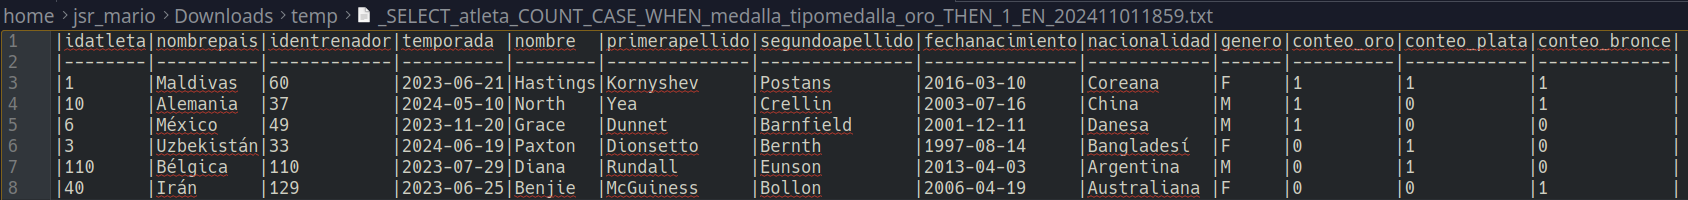
\includegraphics[width=1.05\textwidth]{resources/resultados/10.png}
\end{center}   

Nota: Para este también añadí tuplas manualmente, agregue atletas con medallas en disciplinas que participan; a destacar que aquí creo que hay error de diseño pues medalla guarda atleta y disciplina, pero es complicado verificar si el atleta participa en la disciplina que queremos agregar. \vspace{.3cm}
